\documentclass{article}
\usepackage{rotating}
\usepackage{enumitem}
\usepackage{amsmath}
\usepackage{amssymb}
\usepackage{float}
\usepackage{adjustbox}
\usepackage[utf8]{inputenc}
\usepackage{tikz}
\usepackage{circuitikz} 
\usepackage{float}
\usepackage{lipsum}

\usepackage{graphicx}
\usepackage{subcaption}

\usetikzlibrary{calc}
\usetikzlibrary{positioning,shapes.gates.logic.US}




\usepackage{mathtools}
\usepackage{listings}





\title{ASSIGNMENT 10 }
\author{SUHANI KALRA}

\date{\today} 
\begin{document}

\maketitle





\section{Problem}




\subsection{EC GATE 2014 }

\footnotesize
 In the given circuit, if A is connected to Q1, the operation of the circuit is according to the state diagram. If XOR is replaced with XNOR, then to get the same operation of the circuit which of the following changes has to be done

\subsection{circuit diagram}
\subsection{state diagram}
 \begin{figure}[h]
  \centering
  \begin{subfigure}[h]{0.5\textwidth} \scalebox{0.7}{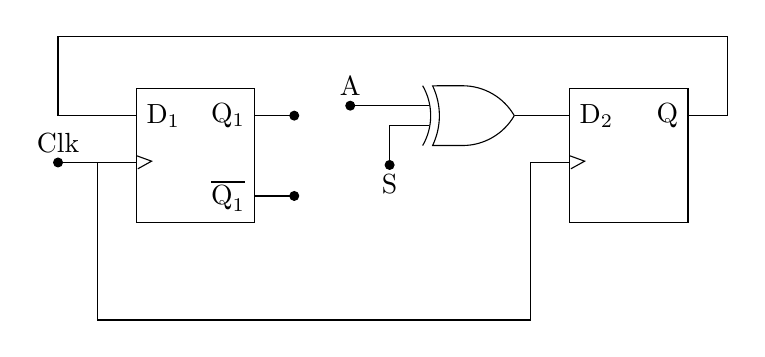
\begin{tikzpicture}[
        GateCfg/.style={
            logic gate inputs={normal,normal,normal},
            draw,
            scale=1.5 
        } 
    ] 

    \draw (-0.5,0)coordinate (A)--++(0:1.5)coordinate (B)--++(90:1.7)coordinate (C)--++(180:1.5)coordinate (D)--cycle;
    \draw ($(B)!0.2!(C)$)node[left]{$\overline{\mbox{Q}_1}$}--++(0:0.5)node[]{}--++(0:0)node[circ]{}; 
    \draw ($(A)!0.8!(D)$)node[right]{D$_1$}--++(180:1)node[]{}--++(90:1)node[]{}--++(0:8.5)node[]{}--++(-90:1)node[]{}; 
    \draw ($(D)!0.5!(A)$)node[]{}--++(-20:0.2)node[]{}--++(-151:0.2)node[]{};
    \draw ($(D)!0.55!(A)$)node[]{}--++(-180:1)node[above]{Clk}--++(0:0)node[circ]{};
    \draw ($(D)!0.55!(A)$)node[]{}--++(180:0.5)node[]{}--++(-90:2)node[]{}--++(0:5.5)node[]{}--++(90:2)node[]{};
    \draw ($(B)!0.8!(C)$)node[left]{Q$_1$}--++(0:0.5)node[]{}--++(0:0)node[circ]{}; 
    
    \draw (5,0)coordinate (A)--++(0:1.5)coordinate (B)--++(90:1.7)coordinate (C)--++(180:1.5)coordinate (D)--cycle;
    \draw ($(A)!0.8!(D)$)node[right]{D$_2$}--++(180:0.5)node[]{};% 
    \draw ($(D)!0.5!(A)$)node[]{}--++(-20:0.2)node[]{}--++(-151:0.2)node[]{};
    \draw ($(B)!0.8!(C)$)node[left]{Q}--++(0:0.5)node[]{}; 
    \draw ($(D)!0.55!(A)$)node[]{}--++(-180:0.5)node[]{}; 
    
    %XOR gate
    \draw (3.7,1.36)node[xor gate US,GateCfg](XOR){};
    
    %connections 
    \draw (XOR.input 1)node[]{}--++(180:1)node[above]{A}--++(0:0)node[circ]{};
    \draw (XOR.input 2)node[]{}--++(180:0.5)node[]{}--++(-90:0.5)node[below]{S}--++(0:0)node[circ]{};
    \draw (XOR.output)node[]{}--++(0:0.2)node[]{};
  
\end{tikzpicture}} 
  \end{subfigure}
   \hfill
  \begin{subfigure}[h]{0.4\textwidth} changed to [h]
    \scalebox{0.6}{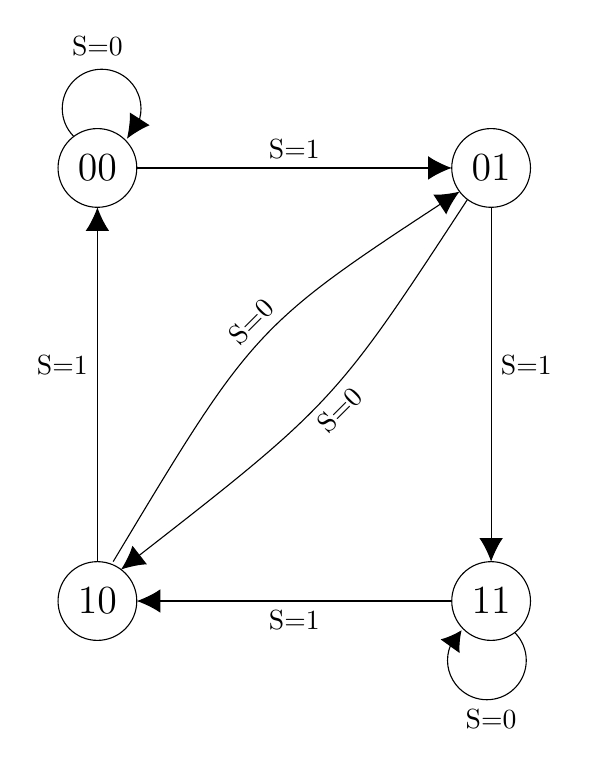
\begin{tikzpicture}
    % first circle and 00
    \draw (0,0)circle(0.5cm)--++(0:0)node[]{\Large00}; 
    
    % arrow loop above 00
    \draw[-{Latex[length=3mm,width=3mm]}] (-0.3,0.4) arc (225:-50:0.5cm); 
    
    % text above loop on 00
    \draw (0,1.3)node[above]{S=0}; 
    
    % arrow from 00 to 01
    \draw[-{Latex[length=3mm,width=3mm]}] (0.5,0)node[]{}--++(0:2)node[above]{S=1}--++(0:2)node[]{}; 
    
    % second circle and 01
    \draw (5,0)circle(0.5cm)--++(0:0)node[]{\Large01}; 
    
    % arrow from 01 to 11
    \draw[-{Latex[length=3mm,width=3mm]}] (5,-0.5)node[]{}--++(-90:2)node[right]{S=1}--(5,-5)node[]{}; 
    
    % third circle and 11
    \draw (5,-5.5)circle(0.5cm)--++(0,0)node[]{\Large11}; 
    
    % loop below 11
    \draw[-{Latex[length=02.5mm,width=3mm]}] (5.3,-5.9) arc (45:-230:0.5cm); 
    
    % text below loop on 11
    \draw (5,-7)node[]{S=0}; 
    
    % arrow from 11 to 10
    \draw[-{Latex[length=3mm,width=3mm]}] (4.5,-5.5)node[]{}--++(180:2)node[below]{S=1}--(0.5,-5.5)node[]{}; 
    % fourth circle and 10
    \draw (0,-5.5)circle(0.5cm)--++(0:0)node[]{\Large10}; 
    
    % arrow from 10 to 00
    \draw[-{Latex[length=3mm,width=3mm]}] (0,-5)node[]{}--++(90:2.5)node[left]{S=1}--(0,-0.5)node[]{}; 
    
    % curved arrow from 10 to 01
    \draw[-{Latex[length=3mm,width=3mm]}] (0.2,-5)..controls (2,-2)..(4.6,-0.3);
    
    % text above curved arrow from 10 to 01
    \begin{rotate}{45}
    \draw (0,-3)node[above]{S=0};
    \end{rotate}
    
    
    \draw[-{Latex[length=3mm,width=3mm]}] (4.7,-0.4)..controls (3,-3)..(0.3,-5.1);
    
    
    \begin{rotate}{45}
    \draw (0,-4.1)node[below]{S=0};
    \end{rotate}


\end{tikzpicture}

} 
  \end{subfigure}
\end{figure}
\text

(a) A should be connected to $\overline{\mbox{Q1}}$\\

(b) A should be connected to Q2\\

(c) A should be connected of Q1 and S is replaced $\overline{\mbox{S}}$  to $\overline{\mbox{Q1}}$ 

\newpage
\large

\section{Solution}
\subsection{basic solution}

\begin{itemize}
\item Initially,

 A=Q1 ,
 D2 = A \oplus S = Q1$\oplus$ S = Q1+ $\overline{\mbox{S}}$Q1

 NOW,\\ XOR GATE is replaced by X-NOR gate\\Let X is unknown \\
So,\\
 D2 = S \odot X =\bar{S}\bar{X} + SX \\
 
 \item But Circits before and after must be same.\\So,\\ D2 = Q $\odot$ S =Q1$\oplus$ S\\
$\overline{\mbox{SX}}$  + SX =$\overline{\mbox{Q1}}$S + $\overline{\mbox{S}}$Q1

\item Then operation does not change.By comparing above, unknown X must be equal to $\overline{\mbox{Q1}}$
\newline i.e. A must be connected to Q1

\subsection{timing diagrams}
%\noindent
% \centering
 \begin{figure}[H]
    \centering
    \scalebox{0.5}{\includegraphics[]{TIMING .pdf}}
    %\includegraphics[width=0.7\linewidth, height=25cm]{TIMING .pdf}
    \caption{}
    \label{}
\end{figure} 


\text to keep Q$_2$ as same as before A=$\overline{\mbox{Q1}}$ and D2 = Q $\odot$ \noindent
\begin{figure}[h]
    \centering
    \includegraphics[width=0.9\linewidth, height=25cm]{TIMING2 .pdf}
   \caption{}
    \label{}
\end{figure}



\end{document}

